\chapter{Puzzles and AI}
\label{puzzles}
In this chapter we provide a background of Sokoban, describing the game rules and its complexity. We then give a short introduction of the classic algorithm \textit{Iterative Deepening A*} and some of its enhancement which have been used in the selected game and that can be found in literature.

\medskip\noindent
Puzzles have been popular since the dawn of mankind, and are known for stimulating brain activity and mental welfare as well as simply being fun. A puzzle is a pastime that consists of a problem or a riddle that tests the ingenuity of those who are called to solve it. There are many types of puzzles that can test different problem-solving skills including logic, pattern recognition, sequence solving, and word completion. The various types of solutions may require structuring a form or creating a certain order. The term puzzle usually refers to single-player games which are enjoyable to play. By definition a puzzle should have a solution which is aesthetically pleasing and gives the user satisfaction in reaching it \cite{journals/icga/KendallPS08}.

\medskip\noindent
In the last decades puzzles have become a more interesting field in computer science due to the fact that finding solutions for them, often requires the recognition of patterns. This makes puzzles suitable to be solved using artificial intelligence agents. A lot of different approaches have been used trying to find a solution to the puzzle solving problem and it has been discovered that specific artificial intelligence methods can work better in some domains rather than in others.

\medskip\noindent
A large amount of different puzzles and artificial intelligence applied to them can be found in literature, and one of the most used algorithm is \textit{Iterative Deepening A*}. This algorithm has been employed to solve different puzzle games such as \textit{n}-Puzzle and Sokoban obtaining good results \cite{journals/icga/KendallPS08}.

\section{Sokoban}\label{sec:sokoban}
Sokoban is a single-player computer game created by Hiroyuki Imabayashi in 1981 and published in December 1982 by Thinking Rabbit, a software house based in Takarazuka, Japan (the japanese name "Sokoban" can be translated as "warehouse keeper"). A level in Sokoban, as shown in Figure \ref{fig:sokobanlevel}, consists of a series of rooms and passageways on a grid, in which are scattered a series of boxes (also called stones) and goals (the dashed area). The number of boxes must match the number of goals.

\begin{figure}[!h]
\centering
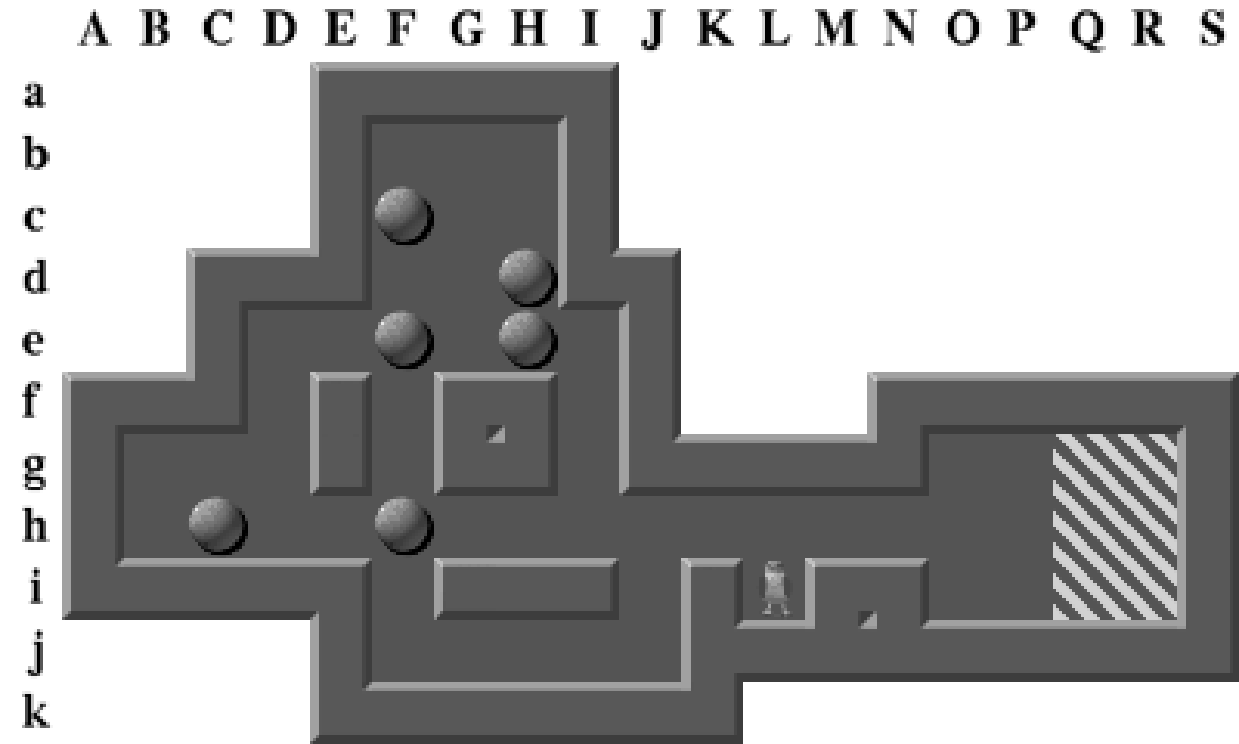
\includegraphics[width=0.7\linewidth]{pictures/sokoban_1.png}
\caption[Example of a Sokoban level]{Example of a Sokoban level \cite{Junghanns99pushingthe}}
\label{fig:sokobanlevel}
\end{figure}

\subsection{Rules}
The goal of the game is to move every box on a goal square. The player controls a character (which we will refer to as the \textit{pusher}) that can move around the level orthogonally on empty squares and goal squares. It cannot cross boxes or walls. If the player tries to move on a square occupied by a box, the box is pushed by one square in the direction of the movement, provided that the target square is either empty or an unoccupied goal. The boxes cannot be pulled, so some moves can be irreversible.

\medskip\noindent
Once every box is on a goal square, the level is solved. In addition to solving the level, the player can also try to find an optimal solution. In Sokoban, the optimality of the solution is usually measured by minimizing one of two metrics:
\begin{itemize}
    \item The total number of pushes, i.e. moves which cause the box to change its position;
    \item The total number of moves, whether they are simple pusher movements or actual box pushes.
\end{itemize}
The canonical metric used is the number of pushes. An optimal solution for a sokoban level can range from a minimum of one push and one move (see level 44 of the Microban set \cite{microban}) to hundreds of pushes and thousands of moves. Sokoban uses a standard format for level files and many level sets have been created by users and enthusiasts\footnote{Most level sets can be found at http://www.sourcecode.se/sokoban/levels}.

\medskip\noindent
One aspect that differentiates it from most puzzles studied in the literature is that an irreversible move can lead to a state that we call \textit{deadlock}, from which no solution can be found. There are two main types of deadlock:
\begin{itemize}
    \item A \textit{simple deadlock} happens when a box is moved on a square from which it cannot reach any goal, regardless of the position of other boxes.
    \item A \textit{freeze deadlock} happens when a box is moved on a non goal square and becomes immovable. That is, when it can't be pushed again. This often includes other boxes that become immovable in turn.
\end{itemize}
Simple deadlocks only depend on the position of a single box, so they can be computed once per level and are fairly easy to identify. Freeze deadlocks instead require interaction between multiple boxes so they must be dealt with at run time. Anyhow, the game is not equipped with deadlock detection mechanisms, so the player can actually continue to play and interact with other boxes despite the deadlock situation. 

\medskip\noindent
In addition to the two main deadlock types, there are other situations that will eventually lead to one of the mentioned deadlocks, but might be recognized earlier. \textit{Corral deadlocks} are defined as a situation in which a portion of the board can't be reached by the player because its access is blocked by boxes and there's no way to get all of those boxes to a goal square. \textit{Bipartite deadlocks} happen when all boxes could still reach a goal, but there's an overlap on the goals they can reach, meaning that not all goals can be occupied at the same time. In order to solve a Sokoban problem, an algorithm (as well as a human player) must be able to recognize these situations early to prune them and reduce the search space. A few examples of deadlocks are represented in Figure \ref{fig:deadlock}.
\begin{figure}[!h]
\centering
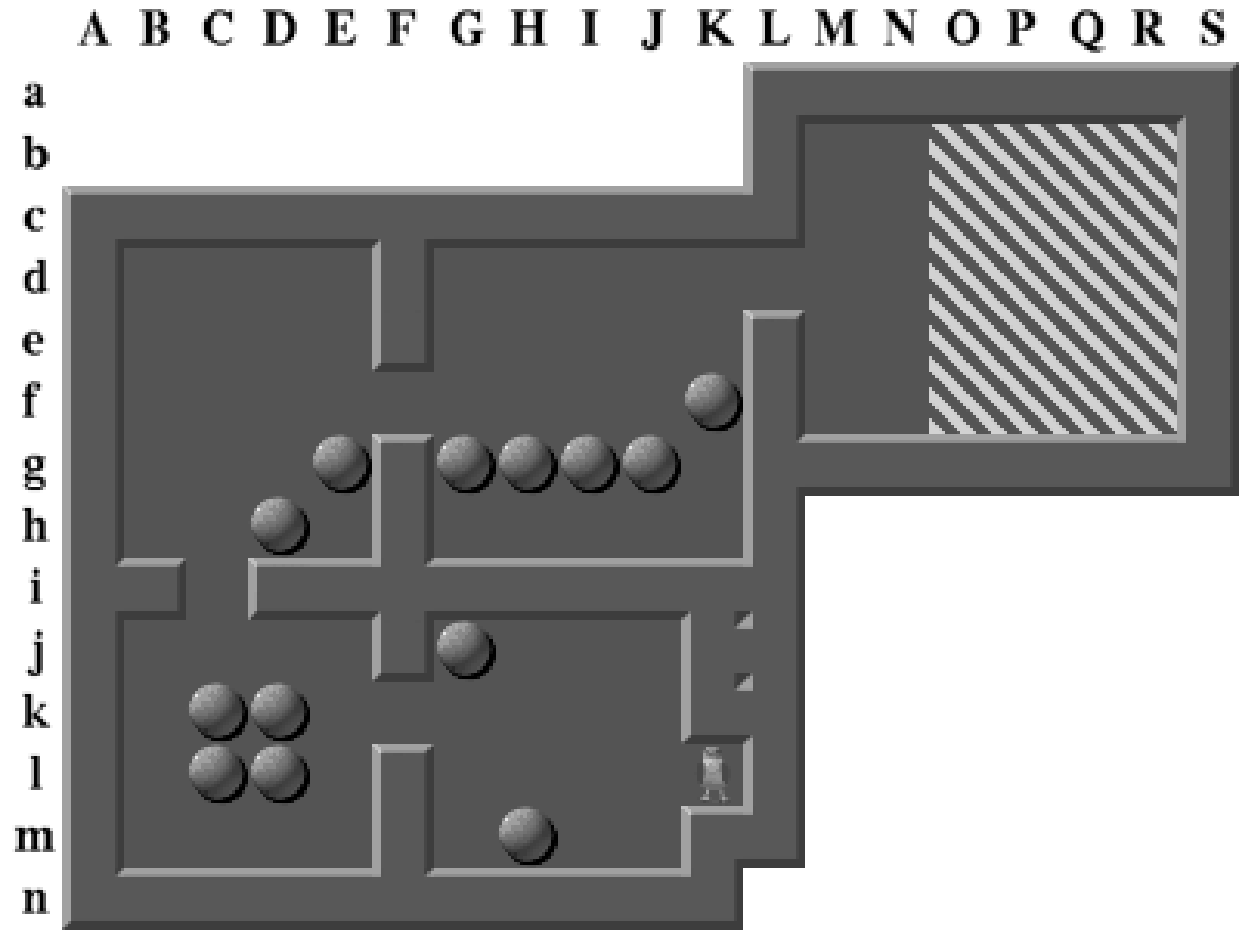
\includegraphics[width=0.7\linewidth]{pictures/sokoban_deadlock.png}
\caption[Deadlock example]{Deadlock examples: upper-left: Corral deadlock; upper-right: Corral deadlock; lower-left: Freeze deadlock; lower-right: Simple deadlock \cite{Junghanns99pushingthe}}
\label{fig:deadlock}
\end{figure}

\subsection{Complexity}
Assuming that our goal is to minimize the number of pushes, we can analyze the game by considering only push moves on boxes that are reachable from the player current position. Considering that in the standard set the number of boxes ranges from 6 to 34 and that we can have up to 4 moves per box, the branching factor can potentially reach a maximum of 136. Of course part of the complexity of Sokoban relies on the constraints that come from the risk of creating deadlocks, so in most of the levels the boxes are densely packed, meaning that the number of available moves is considerably lower. Level 1 (Figure \ref{fig:sokobanlevel}), with only 6 boxes is one of the easiest levels. We can compute an average branching factor $b$ of 3.07, and with a solution length $d$ of 97, the game-tree complexity becomes approximately $10^{47}$. Suppose that we have a similar boxes-to-moves ratio for all levels, with an average number of boxes of 16 and an average solution length of 284.8, we can roughly estimate the average game-tree complexity as $10^{260}$. Since the game rules don't contemplate a limit in the number of moves, and the pusher can retrace its steps, the game length can be considered potentially unlimited. Therefore, to solve a Sokoban puzzle, one should avoid cycles during the search. Junghanns et al. \cite{Junghanns99pushingthe} computed the upper bound for the state-space complexity of Sokoban on a $20\times 20$ board with walls on the perimeter, as $\binom{s}{b}m$ where $s$ is the total number of squares, $b$ is the maximum number of boxes and $m$ is the number of possible pusher positions. This yields a result of $10^{98}$. With an average number of squares of 77 (excluding squares that would cause simple deadlocks) and an average number of boxes of 16, the average state-space complexity of the standard levels suite is approximately $10^{18}$. Sokoban has also been shown to be NP-hard and P-space complete \cite{Pspace-complete97sokobanis} and is considered challenging for both humans and programs.

\section{Iterative Deepening A*}
\textit{Iterative Deepening A*} is one of the most successful methods for puzzle solving that can be found in the literature and it is based on a classical planning approach.

\subsection{Overview}
%\begin{algorithm}
%  \caption{\textbf{A*}}\label{alg:astar}
%  \begin{algorithmic}
%  \Function{Astar}{$\textit{s\textsubscript{0}}$}
%    \State create root node \textit{n\textsubscript{0}} with state \textit{s\textsubscript{0}}
%    \State create queue \textit{frontier} with node $s_0$
%    \While{ \textbf{not} \Call{IsEmpty}{frontier}}
%        \State $n \gets \Call{First}{frontier}$
%        \If{$\Call{IsGoal}{n}$}
%        \State \Return $\Call{BuildSolution}{n}$
%        \EndIf
%        \State $successors \gets \Call{GenerateSuccessors}{n}$
%        \State $\Call{AddToQueue}{frontier, successors}$
%        \State $\Call{Sort}{frontier}$
%    \EndWhile
%    \State \Return $failure$
%    \EndFunction
%  \end{algorithmic}
%\end{algorithm}

\textit{Iterative Deepening A*} (IDA*) is a variant of \textit{Iterative Deepening Depth-First Search} (IDDFS) that relies on heuristic evaluation to determine the threshold for the cut point of the current iteration. It was described by Richard Korf in 1985 \cite{Korf:1985:DIO:4433.4436}. 
IDDFS is an uninformed search method in which a depth limited depth-first search is repeatedly executed with increasing depth limit until a solution is found. At each iteration a full depth-first search is performed until either a solution is found or the entire search tree has been explored up to the depth limit $d$. If no solution has been found, $d$ is increased and the search is repeated. 

\medskip\noindent
The method inherits the low memory complexity of depth first search, while retaining completeness even in presence of unlimited trees. Optimality is preserved if all actions have constant cost.Similarly to IDDFS, IDA* proceeds in a depth-first manner with a depth bound, and once the whole tree for that bound has been explored, the search restarts with an increased bound. Unlike IDDFS, the threshold is not defined in terms of tree depth, but of heuristic evaluation. The method used to determine if the search can continue is based on A* evaluation. A* is an informed search algorithm first proposed in 1968 by Hart et al. \cite{Hart1968} as an improvement over Dijkstra's algorithm for finding the minimum cost path in a weighted graph. At each iteration it explores the node that minimizes
\begin{equation}
    f(n) = g(n)+h(n)
\end{equation}
where $g(n)$ is the cost of reaching node $n$ from the initial node and $h(n)$ is a heuristic estimate of the cost from node $n$ to the goal.

\medskip\noindent
In IDA* as in A*, in order to guarantee the optimality of the solution, the evaluation function $h$ must satisfy the following conditions:
\begin{itemize}
    \item Admissibility: $h(n)<h^*(n)$  with $h^*(n)$ being the perfect heuristic (the actual cost from $n$ to the goal in the optimal solution.
    \item Consistency: $h(n)\leq g(n') + h(n') -g(n)$ where $n'$ is a successor of $n$. 
\end{itemize}
If these condition are satisfied, and a solution is found, that solution is guaranteed to be optimal \cite{Hart1968}.

\subsection{The Algorithm}
IDA* initializes the search threshold as the heuristic value of the initial state $h(n_0)$. It then proceeds in a depth-first exploration until either the value $f(n) = g(n) + h(n)$ exceeds the threshold or there are no more successors. When one of these condition is satisfied, the search returns to the parent node and expands the siblings of the last explored node, exactly like in IDDFS. This produces an asymmetric search tree that grows guided by the heuristic function. The main advantage of this approach with respect to classic A* algorithm is that it runs in space that is linear in the maximum search depth, rather than exponential. Pseudocode for IDA* is showed in Algorithm \ref{alg:idastar}.

\begin{algorithm}
  \caption[IDA*]{\textbf{IDA*}}\label{alg:idastar}
  \begin{algorithmic}
      \Function{IDA*}{$s_0$}
        \State create root node $n_0$ with state $s_0$
        \State create solution $path$ with $n_0$
        \State $threshold \gets \Call{h}{n_0}$
        \While{result not found}
                \State $value \gets \Call{Search}{path,0,threshold}$
            \If{$value = RESULT$}
            \Return $path$
            \EndIf
            \If{$value = \infty$}
            \Return $failure$
            \EndIf
            \State $threshold\gets value$
        \EndWhile
    \EndFunction
    
    \Function{Search}{$path, g, threshold$}
        \State $n\gets \Call{Last}{path}$
        \State $f \gets g+\Call{h}{n}$
        \If{$f>threshold$}
            \Return $f$
        \EndIf
        \If{$\Call{IsGoal}{n}$}
            \Return $RESULT$
        \EndIf
        \State $min\gets\infty$
        \State $successors \gets \Call{GenerateSuccessors}{n}$
        \ForAll{$child$ \textbf{in} $successors$ }
            \State $\Call{Push}{path, child}$
            \State $cost \gets \Call{ActionCost}{child,n}$
            \State $t \gets \Call{Search}{path, g + cost , threshold}$
            \If{$t=RESULT$}
                \Return $RESULT$
            \EndIf
            \State $min\gets \Call{MIN}{min,t}$
            \State $\Call{Pop}{path}$
        \EndFor
        \Return $min$
    \EndFunction
  \end{algorithmic}
\end{algorithm}

\subsection{State of the art}\label{sokobanoptimizations}
IDA* has reached good results in Sokoban \cite{Junghanns99pushingthe} and in the 15-Puzzle (and derivatives) \cite{DBLP:conf/aaai/KorfT96}. 
In the context of Sokoban, the only documented method that can be considered state of the art is the program \textit{Rolling Stone} \cite{Junghanns99pushingthe}. It implements domain independent enhancements \cite{DBLP:journals/pami/ReinefeldM94} to prune the search tree and domain specific enhancements that make use of lower level searches to avoid deadlocks, obtain a tighter lower bound and reduce the search space.

\subsubsection*{Transposition Tables}
Transposition tables consists of data structures used to store information about visited states and are used to avoid cycles during the search and to reduce the branching factor. In Rolling Stone the heuristic evaluation of nodes is stored in the transposition table and updated according to the result of previous iterations. This allows the algorithm to improve the heuristic values and prune sub-trees more efficiently.

\subsubsection*{Move Ordering}
Children of a node are ordered based on the likelihood of leading to a solution. The move ordering scheme proposed was the following:
\begin{enumerate}
    \item \textit{Inertia} moves are considered first. Inertia moves are those moves that preserve inertia, meaning that they act on the same stone as the previous move.
    \item Then all moves that decrease the lower bound are tried (optimal moves), sorted by distance from the stone to its target goal.
    \item Finally, all non-optimal moves are tried, also sorted by distance to target goals.
\end{enumerate}

\subsubsection*{Deadlock Tables}
Deadlock tables make use of pattern database \cite{10.1007/3-540-61291-2_68} to match the current situation to precomputed tables of possible deadlock configurations. The tables are computed offline with all possible combinations of walls, stones and empty squares for a fixed-size region. The deadlock tables are implemented as decision trees, with internal nodes representing subpatterns and leaves representing whether the pattern is a deadlock or not. Junghanns et al. \cite{Junghanns99pushingthe} built two tables for regions of roughly 5x4 squares, that differed in the order the squares in the maze are queried.

\subsubsection*{Tunnel Macros}
A \textit{tunnel} is defined as a part of the maze where the maneuverability of the pusher is restricted to a width of one. These regions cannot have more than one box inside, otherwise they would cause a deadlock. In order to reduce the branching factor, we can collapse all pushes of a box inside a tunnel in a single move that makes the box exit that tunnel.

\subsubsection*{Goal Macros}
When the levels have all goal squares concentrated in a small area, if there are few entrances to this area, the problem can be decomposed in two sub-problems:
\begin{itemize}
    \item moving boxes to the entrances 
    \item placing boxes on goals
\end{itemize}
In some cases these two parts can be solved separately. With Goal Macros, the order in which goal squares must be filled to avoid deadlocks is precomputed, and when a box reaches an entrance the only move it can perform is the Goal Macro, that pushes it directly into its assigned goal.

\subsubsection*{Goal Cuts}
The move pruning of Goal Macros is backpropagated to previous states when a stone is pushed to a square with a Goal Macro at the end without interleaving other stone pushes.

\subsubsection*{Pattern Search}
Pattern search uses sub-problem searches to improve the lower bound and to identify deadlock patterns. It consists of repeated IDA* searches with patterns of more and more boxes. When a deadlock pattern is found, it's saved and used throughout the search in addition to those in the deadlock tables.
The basic algorithm performs the following steps:
\begin{enumerate}
    \item Create a test maze with the same walls and goals configuration but containing only the last moved box.
    \item Try to find a solution to the test maze.
    \item If no solution is found, the pattern is a deadlock. Return pattern.
    \item If a solution is found, add a box that is on a square that is needed for the solution. A square is needed for the solution if either the box or the man had to go through it in the solution found.
    \item If search effort is not exhausted, repeat from 2.
\end{enumerate}
Therefore the pattern search can terminate if the effort is reached, a deadlock was detected or no more stones can be added.
In particular, three types of specialized search has been implemented: 
\begin{itemize}
    \item Deadlock Search: specialized in finding deadlocks, it ignores states that are less likely to contain a deadlock to reduce the cost and be able to include more boxes in the search.
    \item Penalty Search: specialized in finding conflicts between boxes, is not allowed to take shortcuts, hence it might discover patterns ignored by the deadlock search. It's therefore more expensive and it evaluates less boxes with the same search effort.
    \item Area Search: specialized on finding deadlocks, it focuses on areas that are not accessible to the man. It incrementally includes all boxes that surround those areas, trying to find a deadlock. This is similar in concept to the PI-Corral pruning of the YASS solver \cite{yassscribbles}.
\end{itemize}

\subsubsection*{Relevance Cuts}
Relevance cuts is a forward pruning methods that removes moves that are considered not relevant. A move is relevant only if the previous $m$ moves influence it. The influence metric is defined based on the position of the boxes as follows:
\begin{itemize}
    \item Alternatives: The more alternatives exist on a path between two squares, the less the squares influence each other.
    \item Goal-Skew: for a given square $sq$, squares on the optimal path from $sq$ to its goal have a stronger influence than those off the optimal path.
    \item Connection: Two adjacent squares between which a stone can be moved freely influence each other more than two squares between which only the man can move freely.
    \item Tunnel: Influence remains constant inside a tunnel.
\end{itemize}

\subsubsection*{Overestimation}
Overestimation is based on the idea that a good non admissible heuristic might be closer to the optimal value than a poor admissible heuristic. Given the complexity of the problem, non optimal solution are acceptable. Overestimation allows every pattern found during pattern search to increment the lower bound. This will postpone "difficult" situations, giving up optimality but preserving completeness.